% Propósito: enseñar que el nivel de sonoridad en fones y la sonoridad en sones
% son cantidades distintas, y visualizar la duplicación de sones cada 10 phon
% dentro del modelo introductorio.
% Origen: N=2^((L_N-40 phon)/(10 phon)) sone, ecuación
% \eqref{eq:u7-fones-sones}, para L_N>=40 phon. Valores calculados:
% 40, 50, 60, 70 y 80 phon corresponden a 1, 2, 4, 8 y 16 sone.
% Descripción accesible: un gráfico cartesiano muestra nivel de sonoridad entre
% 40 y 80 phon en el eje horizontal y sonoridad entre 0 y 16 sone en el
% vertical. La curva asciende de forma exponencial y pasa por cinco puntos
% rotulados; cada aumento de 10 phon duplica el número de sones.
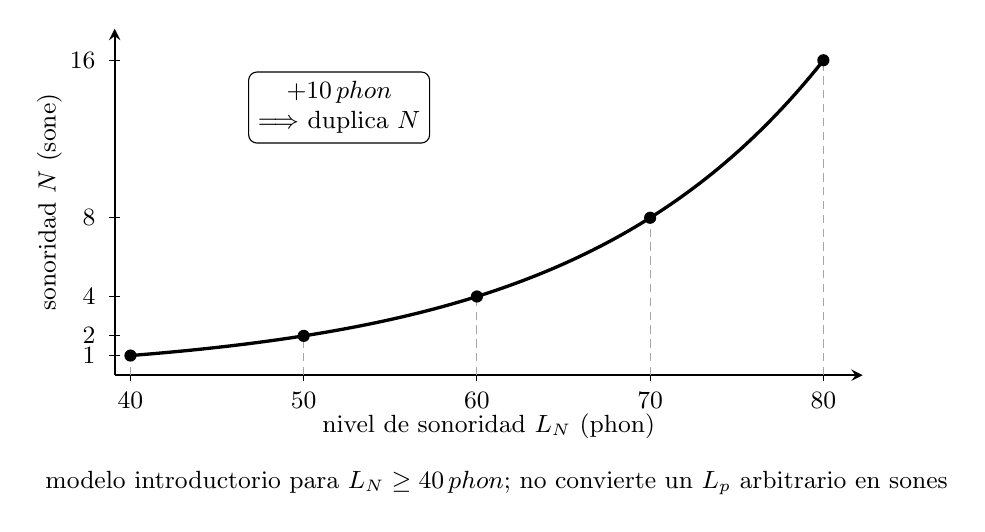
\begin{tikzpicture}[font=\small,>=stealth,x=1cm,y=1cm]
    \draw[->,thick] (1.15,0.75) -- (10.65,0.75);
    \draw[->,thick] (1.15,0.75) -- (1.15,5.15);
    \node at (5.90,0.10) {nivel de sonoridad \(L_N\) (phon)};
    \node[rotate=90] at (0.32,2.95) {sonoridad \(N\) (sone)};

    \foreach \ln/\x in {40/1.35,50/3.55,60/5.75,70/7.95,80/10.15}{
        \draw (\x,0.68) -- (\x,0.82);
        \node[anchor=north] at (\x,0.66) {\(\ln\)};
    }
    \foreach \n/\y in {1/1.00,2/1.25,4/1.75,8/2.75,16/4.75}{
        \draw (1.08,\y) -- (1.22,\y);
        \node[anchor=east] at (1.03,\y) {\(\n\)};
    }

    \draw[very thick,samples=100,domain=40:80]
        plot ({1.35+0.22*(\x-40)},
              {0.75+0.25*pow(2,(\x-40)/10)});

    \foreach \ln/\n/\x/\y in {
        40/1/1.35/1.00,
        50/2/3.55/1.25,
        60/4/5.75/1.75,
        70/8/7.95/2.75,
        80/16/10.15/4.75}{
        \draw[densely dashed,black!35] (\x,0.75) -- (\x,\y);
        \fill (\x,\y) circle (2.2pt);
    }

    \node[draw,rounded corners=3pt,fill=white,align=center] at (4.00,4.15)
        {\(+10\,\text{phon}\)\\
         \(\Longrightarrow\) duplica \(N\)};
    \node[align=center] at (6.00,-0.62)
        {modelo introductorio para \(L_N\geq40\,\text{phon}\);
         no convierte un \(L_p\) arbitrario en sones};
\end{tikzpicture}
